\documentclass[11pt]{report}
\usepackage[utf8]{inputenc}
\usepackage[margin=1in]{geometry}
\usepackage{amsfonts,amsthm,amsmath}
\usepackage{mathtools}
\usepackage{complexity}
\usepackage{fancybox}
\usepackage{parallel}
\usepackage[chapter]{algorithm}
\usepackage{algpseudocode,caption} 
\usepackage{graphicx}
\usepackage{relsize}
\usepackage{tikz}  %TikZ central library is called.
%\usepackage{tkz-graph}
%\usepackage{tkz-berge}
%\usepackage{tikz-network}
\usetikzlibrary{automata,positioning,calc}

\usepackage{tocloft}
\usepackage{palatino}

\RequirePackage[colorlinks=true]{hyperref}
\hypersetup{
  linkcolor=[rgb]{0.3,0.3,0.6},
  citecolor=[rgb]{0.2, 0.6, 0.2},
  urlcolor=[rgb]{0.6, 0.2, 0.2}
}

\usepackage{setspace}
\onehalfspacing


\usepackage{xcolor}
\usepackage{color}
\definecolor{delta}{rgb}{0,0.2,0}
\definecolor{gamma}{rgb}{0,0,0.2}
\definecolor{beta}{rgb}{0.2,0,0}
\definecolor{alpha}{rgb}{0.8,0,0}
\newcommand{\wt}[1]{\widetilde{#1}}
\newcommand{\sse}{\subseteq}
\newcommand{\zo}{\{0,1\}}
\newcommand{\zon}{\zo^n}
\newcommand{\aphantom}{\vphantom{2^2}}
\newcommand{\aaphantom}{\vphantom{2^{2^2}}}
\newcommand{\defn}{\stackrel{\text{\tiny def}}{=}}

% left-right wrappers
\newcommand{\set}[1]{\left\{ #1 \right\}}
\newcommand{\card}[1]{\left|#1 \right|}
\newcommand{\mytilde}[1]{\overset{\sim}{#1}}

% latin
\newcommand{\etal}{\textit{et al}.\@\xspace}
\newcommand{\ie}{i.e.}
\usepackage[all]{xy}
\usepackage{setspace}
\usepackage{amssymb}
\usepackage{amsmath}
\input{preamble.tex}
\usepackage{collect}
\usepackage{wrapfig}
\input{ps-macros.tex}
\renewcommand{\E}{{\mathbb E}}
\title{{\huge CS5130 : Mathematical Tools for Theoretical Computer Science} \\[3mm]
{\LARGE(Scribe Lecture Notes)}\\[1cm]}
\author{{\Large Lecturer : {\sc Jayalal Sarma}} \\[3mm]
Department of Computer Science and Engineering \\[1mm]
Indian Institute of Technology Madras (IITM)\\[1mm]
Chennai, India}
\date{Last updated on : \today}


\begin{document}
\maketitle
\setcounter{page}{1}

\newpage
\pagenumbering{roman}  % Roman numbering in intro portion.
\input{preface.tex}

\newpage
\listofscribe
\newpage
\tableofcontents
\newpage
\listoftodos
\pagenumbering{arabic}
\setcounter{page}{1}
%\setstretch{1.1}

\input{week01.tex}
\input{week02.tex}
\input{week03.tex}
\input{week04.tex}
\input{week05.tex} 
\input{week06.tex}
\input{week07.tex}
\input{week08.tex}
\Lecture{Jayalal Sarma}{Nov 2, 2020}{24}{Algebraic Methods in Combinatorics}{Sampriti Roy}{$\alpha$}{JS}
\section{Introduction}
In this chapter the plan is to switch to algebraic methods in combinatorics and the first structure we are going to explore is the concepts related to group theory. It's essentially going to be presented from the combinatorial side. As, a motivation we can think of the following problems:
\begin{itemize}
\item \emph{How many distinct squares can be there with yellow and blue coloured corners?}
\end{itemize}
Our task is to develop a method to count distinct colourings of such squares out of total $2^4=16$ possible colourings. If we consider the set of all coloured squares to be $\Omega$, there will be some squares that are equivalent to each other under some rotation. As, we are interested in counting distinct colouring, the equivalent squares should not be counted twice.
\paragraph{}
One more question, we can think about is :
\begin{itemize}
\item \emph{How many necklaces can be formed with solid beads and transparent beads? }
\end{itemize}
\paragraph{} 
Based on the colouring of square, we can say that there are total $2^4=16$ possible colourings but there are few operations under which two colourings can be viewed as same. Let's get familiar with such operations:
\begin{itemize}
\item $R_0$ : Rotation by $0^{\circ}$ 
\item $R_{90}$ : Rotation by $90^{\circ}$
\item $R_{180}$ : Rotation by $180^{\circ}$
\item $R_{270}$ : Rotation by $270^{\circ}$
\item $H$ : Horizontal flip
\item $V$ : Vertical flip
\item $D$ : Diagonal flip (bottom left top right)
\item $D'$ : Diagonal flip (bottom right top left)
\end{itemize}
Now, let's consider all the above set of operations together to be :
\begin{align*}
G&=\{R_0,R_{90},R_{180},R_{270},H,V,D,D'\} 
\end{align*}
We will see that the elements of set $G$ are inter related with each other. If we apply two operations from $G$, one after another, we will get the result of applying an operation from $G$ itself. Let's verify it:
\begin{itemize}
\item Rotate the square two times horizontally, it will result rotating it by $0^{\circ}$. That is $H.H=R_0$
\item Rotate the square two times diagonally, it will result rotating it by $0^{\circ}$. That is $D.D=R_0$
\item Rotate the square two times vertically, it will result rotating it by $0^{\circ}$. That is $V.V=R_0$
\item Rotate the square two times by $180^{\circ}$, it will result rotating it by $0^{\circ}$. That is $R_{180}.R_{180}=R_0$
\item Rotate the square by $90^{\circ}$ first then rotate it by $180^{\circ}$, it will result rotating by $270^{\circ}$. That is $R_{90}R_{180}=R_{270}$
\item  Rotate the square by $90^{\circ}$ first then rotate it by $270^{\circ}$, it will result rotating by $0^{\circ}$. That is $R_{90}R_{270}=R_{0}$
\item Rotate the square by $90^{\circ}$ first then rotate it vertically, it will result rotating diagonally. That is $R_{90}.V=D $
\end{itemize}
\section{Incremental definition of Group}
Consider a set $G$ with binary operation $\circ$. Now, take any two elements of $G$ and apply the operation, a natural question to ask is whether we will get any element from the set $G$ or not. We will answer this question along with other related questions and finally move on to the definition of Group incrementally.
\begin{itemize}
\item \emph{Groupoid} : Let $a,b\in G$. If $a\circ b\in G$, then $G$ is \emph{Closed} under the operation $\circ$. And $G$ is called \emph{Groupoid}. We can easily verify that our example set $G$ is a \emph{Groupiod}.
\item \emph{Semigroup} : $a,b,c\in G$; if $a\circ(b\circ c)=(a\circ b)\circ c $, then $G$ is \emph{associative} under $\circ$ or, the order of $\circ$ does not matter. If a groupoid is associative, it is called \emph{Semigroup}. We can try out and check that our example set $G$ is associative and so it is a \emph{Semigroup}.
\item \emph{Monoid} : $\forall a\in G $, if there is an $e\in G$ such that $a\circ e=e\circ a\forall $, $e$ is called identity element. A Semigoup with identity is called \emph{Monoid}. In our example set $G$, $R_0$ is the identity element, so it is a \emph{Monoid}.
\item \emph{Group} : $\forall a\in G$ if $ \exists b\in G $ such that $a\circ b=b\circ a=e $; where $e$ is identity element, $b$ is called the \emph{inverse} of $a$. A Monoid with inverse element is called a \emph{Group}. In our example set $G$, $R_{180}$ is it's own inverse, $H$ is it's own inverse and we can try out that every element has it's inverse and so it is a \emph{Group}.
\end{itemize}
Hence, we can conclude that $G=\{R_0,R_{90},R_{180},R_{270},H,V,D,D'\}  $ is not just a set, rather it has more structural properties. $(G,\circ) $ is a \emph{Group}. Now, we are ready to define \emph{Group} formally.
\begin{definition}
$(G,\circ)$ is a group if it satisfies closure, associativity and it has identity and inverse element.
\end{definition} 
\textbf{Example1} : Let's consider $\mathbb{Z}_p=\{0,1,...,p-1\} $ where $p$ is a prime number. Define the operation to be $+ \  mod \ p $. Let's verify whether $(\mathbb{Z}_p,+ \ mod \ p) $ is a group or not:
\begin{itemize}
\item \emph{Closure} : $\forall a, b\in \mathbb{Z}_p; a+ \ mod \ p\in \mathbb{Z}_p$. So, $\mathbb{Z}_p$ is closed under the operation $+ \ mod \ p$
\item \emph{Associativity} : As modulo arithmetic is associative, $\mathbb{Z}_p$ is associative under $+ \ mod \ p$
\item \emph{Identity} : $0$ is the identity element for all elements in $\mathbb{Z}_p$. 
\item \emph{Inverse} : For any element $a\in \mathbb{Z}_p$, $(p-a)$ will be the inverse of $a$.
\end{itemize}
Hence, $(\mathbb{Z}_p,+ \ mod \ p) $ is a group.
\paragraph{}
Let's check whether $(\mathbb{Z}_p,\times \ mod  \ p) $ is group or not:
\begin{itemize}
\item \emph{Closure} : $\forall a, b\in \mathbb{Z}_p; a\times \ mod \ p\in \mathbb{Z}_p$. So, $\mathbb{Z}_p$ is closed under the operation $\times \ mod \ p$
\item \emph{Associativity} : As modulo arithmetic is associative, $\mathbb{Z}_p$ is associative under $\times \ mod \ p$
\item \emph{Identity} : $1$ is the identity element for all elements in $\mathbb{Z}_p$
\item \emph{Inverse} : The element $0$ does not have any inverse.
\end{itemize}
Hence, $(\mathbb{Z}_p,\times \ mod  \ p) $ is not a group but it is a \emph{Monoid}.
\paragraph{}
Consider the group $\mathbb{Z}_p^* $ under the operation $\times \ mod  \ p $; for example we can verify that $(\mathbb{Z}_p^*,\times \ mod  \ p) $ satisfies closure, associativity, identity and inverse properties. Hence, $(\mathbb{Z}_p^*,\times \ mod  \ p) $ is a group.\\
\textbf{Exercise} : Use \emph{pigeon hole principle} to prove that every element has it's inverse in  $(\mathbb{Z}_p^*,\times \ mod  \ p) $.
\paragraph{}
\textbf{Example2} : Set of bijection from $\{1,2,...,n\} $ to $\{1,2,...,n\}$ forms a group under composition ($\circ $).
\begin{itemize}
\item \emph{Closure} : Composition of two bijections is bijection
\item \emph{Associative} : Using function composition property, if $f,g,h$ are functions, $f\circ(g\circ h)=(f\circ g)\circ h$
\item \emph{Identity} : Identity function will be there
\item \emph{Inverse} : Every element will have inverse
\end{itemize}
Hence, set of bijections $(S_n,\circ) $ forms a group.
\section{Group (abstractly)}
So far, we have seen the definition of a group $G$, under some operation $\circ$. Now, we will move on the definition of \emph{Subgroup}.
\begin{definition}
Let $(G,\circ) $ be a group. $H\subseteq G$ is said to be a subgroup if $H$ forms a group by itself with respect to the same operation $\circ$. A subgroup of $G$ is denoted by $H\leq G$. 
\end{definition}
\textbf{Example} : $(\mathbb{Z}_{15},+ \ mod \ 15) $ is a group. Consider $H=\{0,3,6,9,12\}$. $H\subseteq G$ and $H$ satisfies closure, associativity, identity, inverse and so it forms a group under $+ \ mod \ 15 $, so $H\leq G$.
\subsection{Subgroup}
Consider a group $G$ and $H\leq G$. Let's take an element $g$ from $G\setminus H$ and multiply it with $H$, define:
\begin{align}
Hg=\{hg|h\in H\}
\end{align} 
\begin{observation}
If $g\in H$; then $Hg\subseteq H$ as $H$ is closed by itself. 
\end{observation}
It's not just $Hg\subseteq H$; something more is true. For that, we will have the following claim
\begin{claim}
$|Hg|=|H|$ when $g\in H$
\end{claim}
\begin{proof}
$\forall h_1\neq h_2\in H$, we need to argue that $h_1g\neq h_2g$. Or multiplication by $g$ is actually a bijection.\\
Let's prove it by contradiction and let $\forall h_1\neq h_2\in H$
\begin{align*}
h_1g&=h_2g\\
h_1&=h_2gg^{-1}\\
h_1&=h_2
\end{align*}
Hence, we get a contradiction. So, $h_1g\neq h_2g$
\end{proof}
Now, let's move on to the following claim
\begin{claim}
$\forall g_1,g_2$; if $Hg_1\cap Hg_2\neq \emptyset $; then $Hg_1=Hg_2$. In other words, if $Hg_1$ and $Hg_2$ are overlapping, then they are same.
\end{claim}
\begin{proof}
Let $g_1,g_2\in G$. Suppose $g\in Hg_1\cap Hg_2$
\begin{align*}
\exists h\in H; g&=hg_1\\
\exists h'\in H; g&=h'g_2
\end{align*}
Now, combining the above two,
\begin{align*}
hg_1&=h'g_2\\
g_1&=h^{-1}h'g_2
\end{align*}
Now, we are ready to prove $Hg_1\subseteq Hg_2$\\
Consider, any element in LHS $h''\in H $, substituting $g_1$, we get:
\begin{align*}
h''g_1&=h''h^{-1}h'g_2\\
&=h'''g_2
\end{align*}
Hence, any element in LHS is in RHS. Similarly, we can prove $Hg_2\subseteq Hg_1$. So, $Hg_1=Hg_2$.
\end{proof}
\paragraph{}
So, we can argue that the multiplication of $H$ by other elements will result in translation of $H$ which are kind of tiling of group $G$. It does not mean that every $g_i$ will give different tiles, but if they have common element, they are same. One interesting feature is that all such tiles will have equal size. One natural question is can there be any element that is not in any tiling? Yes, there can be. For example, $\forall g\in G, g\in Hg$ because $H$ contains identity as it is subgroup. So,$g$ is an element of $Hg$ always. So, every element $g$ will be there in some tile for sure. If there are total $k$ tiles, we argue that:
\begin{align*}
|G|&=k.|H|
\end{align*}
\begin{theorem}
Lagrange's Theorem : The size of a subgroup $|H$ must divide the size of a group $|G|$.
\end{theorem}
 For example, A group of size $100$ can not have a subgroup of size $99$. In fact it can only have subgroup of size at most $50$. Any group with prime number of elements, can not have any non-trivial subgroup. So, \emph{Lagrange's Theorem} is the example of algebraic structure implying combinatorial bounds.


\Lecture{Jayalal Sarma}{Nov 4, 2020}{25}{A step towards Polya's Theory }{Sampriti Roy}{$\alpha$}{JS}
\section{A quick recap}
 In last lecture, we started with a problem of counting number of distinct colourings when the corner of a square are coloured with $2$ colours. We defined a set $G=\{R_0,R_{90},R_{180},R_{270},H,V,D,D'\} $ that acts on set of all possible $2$-coloured squares and some of them are equivalent under these operations. We have also talked about the definition of subgroup $(H)$ of a group $(G)$ and defined that for $g\in G\setminus H$, $Hg=\{hg: h\in H \}$. This $Hg$ is called \emph{coset} of $H$ in $G$. 
We have also seen that if any two cosets overlap, they have to be same. We have also talked about \emph{Lagrange's Theorem}. In this chapter the plan is to understand \emph{Polya's Theory}. We will complete it only in next lecture but we will do a step towards it. The step is known to be \emph{Burnside's Lemma}. 
\section{The abstract problem of counting distinct 2-coloured squares}
 $\Omega$ be the set of all $2$-coloured squares. There $|\Omega|=2^4=16$ possibilities. Our task is to count to number of distinct colourings among $\Omega$. Let's define the equivalence between two coloured squares formally:
 \begin{definition}
 Let $\alpha,\beta\in \Omega$, if $\exists g\in G$ such that the action on $g$ on $\alpha$ returns $\beta$, or $\alpha^g=\beta$; then we say $\alpha$ and $\beta$ are equivalent, $\alpha\sim \beta$.
\end{definition}
The relation $\sim$ between $\alpha$ and $\beta$ satisfies the following properties:
\begin{itemize}
\item \emph{Reflexive} : $\alpha\sim \alpha$
\item \emph{Symmetric} : $\alpha\sim \beta\rightarrow \beta\sim \alpha$; if the action of $g$ makes the transformation from $\alpha$ to $\beta$, then $g^{-1}$ will make the transformation from $\beta$ to $\alpha$. For example, $R_{90}$ transform $\alpha$ to $\beta$, $R_{270}$ will transform $\beta$ to $\alpha$.
\item \emph{Transitive} : If $\alpha\sim \beta$ by the action $g_1$, $\beta\sim \gamma$ by the action $g_2$; then the action of $g_1g_2$ (composition of $g_1,g_2$) will transform $\alpha\sim \gamma$.
\end{itemize}
Hence, $\sim$ is an equivalence relation and it splits the set $\Omega$ into set of equivalence classes.
\subsection{Orbit and Stabilizer}
The action of $g$ on $\Omega$, partitions $\Omega$ into different equivalence classes but their sizes need not be equal. This equivalence classes are called \emph{Orbit}. In our context, among set of all possible $2$-colourings of a square, we don't want to count equivalent squares twice. In other words, the abstract problem that we are interested to study is to count the number of orbits of $\Omega$. First, we are going to study the sizes of the orbits and using them we will have a mechanism to count them. Let's define the following
\begin{definition}
$Orbit_G(\alpha)=$ orbit of $\alpha$ under the action of $G$ on $\Omega$
\begin{align*}
Orbit_G(\alpha)&=\{\beta:\exists g\in G \ s.t \ \alpha^g=\beta \}
\end{align*}
\end{definition}
Now, we are ready to define \emph{Stabilizer} of $\alpha$ on an action of $G$. Let, $g\in G$ is acting on $\Omega$. Let $\alpha\in G$, which are  the elements in $G$ that fixes $\alpha$? i.e, the elements in $G$ that takes $\alpha$ to itself. 
\begin{definition}
Stabilizer of an element $\alpha$ is a subset of $G$, which acts on $\alpha$ and takes it back to itself.
\begin{align*}
Stab_G(\alpha)&=\{g\in G: \alpha^g=\alpha \}
\end{align*}
\end{definition}
We will see few examples of stabilizer to make it more clear. 
\begin{itemize}
\item \emph{Example 1} : A simple example we can think of in our square setting is that, let $\alpha$ be the square where all the corners are coloured yellow. Now, we can easily conclude that any operation from the group $G$ can fix $\alpha$, i.e, no matter which action we are performing, $\alpha$ will be $\alpha$ itself. So, the stabilizer of $\alpha$ is the entire group $G$.
\item \emph{Example 2} : Let's think of another $\alpha$ where bottom left and top right corners are coloured blue and the other two are coloured yellow. Now, we can verify that the operations that fixes $\alpha$ are : $\{R_0,R_{180},D,D' \} $. 
\end{itemize}
An interesting observation is that stabilizers inside $G$ are not only subset of $G$, they are actually subgroup of $G$. Let's prove the argument formally,
\begin{claim}
$$Stab_G(\alpha)\leq G$$
\end{claim}
\begin{proof}
Fix an $\alpha$ and verify the following :
\begin{itemize}
\item \emph{Closure} : If $g_1,g_2\in Stab_G(\alpha)$, then $g_1g_2\in Stab_G(\alpha)$. As, $g_1,g_2$ are fixing $\alpha$, then their composition will also fix $\alpha$.
\item \emph{Associativity} : As the operations performed are subset of $G$, associativity is inherited in $Stab_G(\alpha)$.
\item \emph{Identity} : Identity fixes every element, in particular it fixes $\alpha$. So, identity element is present in $Stab_G(\alpha)$.
\item \emph{Inverse} : If an element $g$ fixes $\alpha$, then $g^{-1}$ will also fix $\alpha$. So, inverse element is always present in $Stab_G(\alpha)$. For example,   if $R_{90}$ fixes a coloured square, then $R_{270}$ will also fix the same square.
\end{itemize}
Hence, $Stab_G(\alpha)\leq G$
\end{proof}
There is a combinatorially useful relation between size of the stabilizer and the size of the of $\alpha$. Let's define the following lemma;
\begin{lemma}
\textbf{Orbit-Stabilizer Lemma} : $$\forall\in \Omega;|Orbit_G(\alpha)|.|Stab_G(\alpha)|=|G|$$
\end{lemma}
We will prove this lemma formally in next lecture, but here we are going to draw a outline of the thought process to prove this lemma.
\paragraph{}
\emph{Proof Idea} : Let $Stab_G(\alpha)$ be denoted by $H$. We have already proved that $Stab_G(\alpha)$ is a subgroup of $G$. Using \emph{Lagrange's theorem} we can say that $$|G|=k.|Stab_G(\alpha)|$$
Where $k$ is the number of cosets $H$ in $G$. So, it is sufficient to prove that number of cosets $H$ in $G$ is exactly $|Orbit_G(\alpha)|$. We will show a bijection that for every element in the orbit of $\alpha$, there is a way to associate a corresponding coset with it. Hence, the number of coset in $Stab_G(\alpha) =|Orbit_G(\alpha)|$. Now, we will quickly define the bijection:
\paragraph{}
Consider any $\beta\in Orbit(\alpha)$; it means $\exists g\in G $ s.t. $\alpha^g=\beta $. Now, coset corresponding to $g$ is $Hg$. We required to show the following:
\begin{itemize}
\item \emph{Well definedness} : There could be many $g\in G$ which makes $\alpha$ to $\beta$. We need to argue that no matter which $g\in G$ we choose, we will end up by getting the coset $Hg$.
\item \emph{Injection} : For $\beta\neq \beta'\in Orbit(\alpha)$; there is $g,g'\in G$ where $\alpha^g=\beta,\alpha^{g'}=\beta'$; we will end up by getting two different cosets, i.e., $Hg\neq Hg' $.
\item \emph{Surjection} : To show that for any coset we have corresponding element in the orbit of $\alpha$.
\end{itemize}
An interesting observation we can make from the above lemma is that if the size of a group is any prime number then either $|Stab_G(\alpha)|$ is same as $|G|$ and $|Orbit_G(\alpha)|=1$ or $|Stab_G(\alpha)|=1$ and $|Orbit_G(\alpha)|$ is same as $|G|$. But, we are not interested in individual sizes of orbits but we want to count the number of orbits. We will use the \emph{Orbit-Stabilizer lemma} to define the following lemma to show that if we have a handle on the size of orbits then we can have a handle on the number on number of orbits as well. First, we will define the following:
\begin{definition}
\textbf{Fix Points} : If $G$ is acting on $\Omega$, fix points of a group element are those elements on $\Omega$ that are fixed by $g$.
\begin{align*}
fix(g)&=\{\alpha\in \Omega: \alpha^g=\alpha \}
\end{align*}
\end{definition}
Now, we are ready to state the following lemma:
\begin{lemma}
\textbf{Burnsides Lemma} : 
\begin{align*}
\#of \ orbits \ &=\frac{1}{|G|}\sum_{g\in G}|fix(g)|
\end{align*}
\end{lemma}
\begin{proof}
The proof is a classic proof by double counting method. Let's define the set
\begin{align*}
S&=\{(g,\alpha): g\in G, \alpha\in \Omega; \alpha^g=\alpha \}
\end{align*}
We will estimate $|S|$ in two different ways:
\begin{itemize}
\item Answer $1$ : For each $g$ count number of different $\alpha$ that are fixed by $g$.
\begin{align*}
&\sum_{g\in G} (\#of \ \alpha \ s.t \ \alpha^g=\alpha)\\
&=\sum_{g\in G}|fix(g)|
\end{align*}
\item Answer $2$ : For each $\alpha\in \Omega$, count number of different $g$ that fixes $\alpha$.
\begin{align*}
&\sum_{\alpha\in \Omega} (\#of \ g \ s.t \ \alpha^g=\alpha)\\
&=\sum_{\alpha\in \Omega}|Stab_G(\alpha)|\\
&=\sum_{\alpha\in \Omega}\frac{|G|}{|Orbit_G(\alpha)|}\\
&=|G|.\sum_{\alpha\in \Omega}\frac{1}{|Orbit_G(\alpha)|}\\
\end{align*}
Let us consider the orbits of $\Omega$ are denoted by $\{\Omega_1,\Omega_2,...\}$. Then the above expression becomes,
\begin{align*}
&=|G|.(\sum_{\alpha\in \Omega_1}\frac{1}{|\Omega_1|}+\sum_{\alpha\in \Omega_2}\frac{1}{|\Omega_2|} )\\
&=|G|.(\#of \ orbits)
\end{align*}
\end{itemize}
Equating Answer $1$ and $2$, we get:
\begin{align*}
|G|.(\#of \ orbits)&=\sum_{g\in G}|fix(g)|\\
\#of \ orbits&=\frac{1}{|G|}\sum_{g\in G}|fix(g)|
\end{align*}
\end{proof}
\section{Counting number of distinct coloured square using Bernsides Lemma}
We we apply Bernsides lemma to our example problem to count number of distinct coloured squares in $\Omega$. For that, first we have to compute $|fix(g)|$ for each $g\in G$. Where $G=\{R_0,R_{90},R_{180},R_{270},H,V,D,D'\}  $.
\begin{itemize}
\item $g=R_0$; all the coloured squares in $\Omega$ are fixed by $g$. So, $|fix(R_0)|=|\Omega|=16$
\item $g=R_{90}$; the squares whose all corners are either blue or yellow will be fixed by $g$. So, $|fix(R_{90})|=2 $
\item $g=R_{180}$; total $4$ squares will be fixed  by $g$. So, $|fix(R_{180})|=4 $
\item $g=R_{270}$; the number of squares that will be fixed are same as $R_{90}$. Because, if a square is fixed by $R_{90}$, it will be fixed by it's inverse as well. So, $|fix(R_{270})|=2 $
\item $g=H$; it will fix the squares where the upper half and lower half corresponding to the horizontal plane (line towards the middle of the square) will be coloured with same colour. so, $|fix(H)|=4 $
\item $g=V$; the number of squares will be same as that are fixed by $H$. so, $|fix(V)|=4 $
\item $g=D$; consider one diagonal and corresponding to it the upper half and lower half will be coloured with same colour, there are $2$ ways to do it and for each such colour the diagonal can be coloured in $4$ ways. So, $|fix(D)|=8 $
\item $g=D'$; the number of squares will be same as that are fixed by $D$. So, $|fix(D')|=8$
\end{itemize}
Using Bernsides lemma,
\begin{align*}
\#of \ orbits \ in \ \Omega&=\frac{1}{8}(16+2+4+2+4+4+8+8)\\
&=6
\end{align*}
So, out of the $16$ total colourings $6$ of them are in-equivalent to each other. To simulate the thought process, here is an exercise:
\emph{Exercise} : Consider all $2$-coloured squares and the set of operations that are acting on it are defined by $G'=\{R_0,R_{90},R_{180},R_{270}\}$, i.e. we are not worried about the $H,V,D,D'$ rotations. Under this operations count the number of distinct $2$-coloured squares. 
\\

\Lecture{Jayalal Sarma}{Nov 11, 2020}{26}{Another step towards Polya's Theory }{Achyuth Prakash}{$\alpha$}{JS}
\section{A quick recap}
 In last lecture, we defined and proved the orbit-stabilizer lemma and Lagrange's theorem. In this chapter the plan is to better understand \emph{Polya's Theory} by going through a further example. 

\section{Example 2: Coloring faces of a cube}
Let us consider coloring the faces of a cube with $2$ colors. As before we define, $\Omega$ as the set of all possible colorings. There are $6$ faces, and each can can be colored with $2$ colors, thus we have $|\Omega| = 2^6 = 64$.
\\
Next we define the set of 'operations', $G$ which can act on elements on $\Omega$. What are the different possible operations? We list them and simultaneously compute $|fix(g)|$:
\\
Here is the labelled cube for reference:
\\
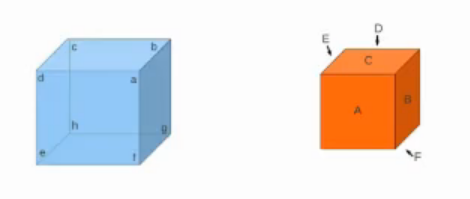
\includegraphics[]{./images/cube.png}
\\
The different operations are:
\begin{itemize}
\item $R_0$ : Rotation by $0^{\circ}$, i.e. identity. Since all elements of $\Omega$ when acted upon by $R_0$ give back the same element, we get $|fix(g)| = 64$.

\item $R_1$ : Rotation by $180^{\circ}$ w.r.t axis through the center of the opposite faces. (Observe that there are $3$ pairs of such faces). Now consider $2$ such faces, $A, D$. If we rotate the cube as per $R_1$, how many elements of $\Omega$ remain unchanged? 
\\
Consider the faces $A, D$. They can be colored with any color each. Thus, there are $2*2 = 4$ choices. Now, for the other faces, consider $C, F$. These $2$ must be colored with the the same color(because they exchange places) Thus there are $2$ choices for $C, F$ together. Similarly for $B, E$. Thus in total, there are $2^4 = 16$ elements which belong to $fix(g)$.

\item $R_2$ : Rotation by $90^{\circ}$ w.r.t axis through the center of the opposite faces. Observe that there are $3$ pairs of such faces. Again let us compute $|fix(g)|$.
\\
Consider the faces $A, D$. They can be colored with any color each. Thus, there are $2*2 = 4$ choices. Now, for the other faces, they all must be colored with the same color, because, $C \rightarrow B$, $B \rightarrow F$, $F \rightarrow E$, and $E \rightarrow C$. Thus, there are $2$ choices for $B, C, E, F$ together. Hence, $|fix(g)| = 2^3 = 8$.

\item $R_3$ : Rotation by $270^{\circ}$ w.r.t axis through the center of the opposite faces. Observe that there are $3$ pairs of such faces. Let us compute $|fix(g)|$.
\\
Since this is the exact opposite of the previous case, by symmetry, $|fix(g)| = 8$.

\item $R_4$ : Rotation by $180^{\circ}$ w.r.t axis through the midpoints of opposite edges. Observe that there are $6$ pairs of such edges, i.e. $(de, bg),\ (af, ch),\ (ad, hg),\ (cb, ef),\ (ab, eh),\ (cd, fg)$. To compute $|fix(g)|$, 
\\
Suppose we do the rotation w.r.t the edges $(de, bg)$. then observe that, now $F$ is now the top face, and $A$ occupies the place where $E$ was initially, similarly, $B$ and $D$ swap places. Thus there are $2$ choices together for $C, F$, $2$ choices for $A, E$ and $2$ for $B, D$, giving $8$ choices overall.
Thus, $|fix(g)| = 8$.

\item $D$ : Diagonal flip by $120^{\circ}$ w.r.t axis through the centers of opposite corners. First, note that there are $4$ pairs of opposite corners. To compute $|fix(g)|$,
\\
Consider the vertex $b$. If we flip the cube along $b$ by $120^{\circ}$, then the face $B \rightarrow C$, i.e. $B$ now occupies the initial position of $C$, $C \rightarrow D$ and $D \rightarrow B$. Thus together, for $B, C, D$ there are $2$ choices. Similarly for $A, E, F$. Thus totally we get $2*2 = 4$ possibilities, and $|fix(g)| = 4$.

\item $D'$ : Diagonal flip by $240^{\circ}$ w.r.t axis through the centers of opposite corners. First, note that there are $4$ pairs of opposite corners. To compute $|fix(g)|$,
\\
By symmetry, this is the opposite/complementary operation of the previous one, i.e. flip by $240^{\circ}$ = flip by $120^{\circ}$ in the other direction. Thus, $|fix(g)| = 4$.
\end{itemize}

Thus totally there are $1 + 3*3 + 6 + 4*2 = 24$ operations in $G$.

Now, if we apply the formula to calculate the number of orbits, we get:
$$\#of \ orbits \ in \ \Omega =\frac{1}{24}(64 + 3*16 + 3*8 + 3*8 + 6*8 + 4*4 + 4*4) = 10$$

Therefore, we observe that out of the $64$ colorings, $10$ of them are in-equivalent.

\section{Cycle Index}
We now introduce and define the notion of cycle indices. Let $G$ be the set of some permutations on $\Omega$. Let us decompose $g \in G$ into a collection of disjoint cycles. 
\\
For example, let $n = 5$. Consider the permutation $3, 1, 2, 5, 4$ we write this as $(1, 2, 3)\ (4, 5)$, i.e. this denotes $1 \rightarrow 2$, (i.e. $1$ goes to position $2$), $2 \rightarrow 3, 3 \rightarrow 1$ and so on. 
\\
Similarly, the identity permutation, $1, 2, 3, 4, 5$ would be written as $(1)(2)(3)(4)(5)$.
\begin{definition}
\textbf{Type of permutation $\pi$} : A permuatation $\pi$ is said to be of type $(b_1, b_2, \ldots b_m)$ if $b_i$ represents the number of $i$ length cycles in the cycle representation of $\pi$.
\end{definition}

For example if $\pi = (1, 2, 3)\ (4, 5)$ then it is of type $(0, 1, 1, 0, 0)$, because there are no $1$ length cycles, $\implies b_1 = 0$, one $2$ length cycle, i.e. $4 \rightarrow 5 \rightarrow 4 \implies b_2 = 1$, and one $3$ length cycle.

Now, corresponding to type $(b_1, b_2, \ldots b_m)$ consider the monomial $x_1^{b_1}\ x_2^{b_2} \ldots x_m^{b_m}$. Using these terms we define a polynomial as follows:
\begin{definition}
Cycle index polynomial of $G$:
\end{definition}
$$P(x_1, x_2, \ldots x_m) = \frac{1}{|G|} \sum_{g \in G} x_1^{b_1}\ x_2^{b_2} \ldots x_m^{b_m}$$ where $(b_1, b_2, \ldots b_m)$ is the cycle type of $g$.
\\
We observe that the above polynomial generalises the Burnside's lemma because we can now substitute the number of possible colors say $2$ in place of $x_1, x_2, \ldots x_m$. Thus, this theorem is much more versatile.
\\

\Lecture{Jayalal Sarma}{Nov 12, 2020}{27}{Polya's Theory - Part 1}{Achyuth Prakash}{$\alpha$}{JS}
\section{Quick Recap}
In the last lecture, we went through another example(of coloring the faces of a cube) and defined the cycle index polynomial of $G$.
\\
Consider an example:
Let $G$ be a group such that $G = \{e, (1, 2),\ (3, 4),\ (1,2)(3,4)\} \le S_4$
i.e., $G$ is a subgroup of $S_4$.
\\
Thus, let us write down the cycle index polynomial of $G$:
$$P(x_1, x_2, x_3, x_4) = \frac{1}{4} (x_1^4 + x_1^2x_2 + x_1^2x_2 + x_2^2)$$
We get the RHS because $e$ has $4$ length $1$ cycles, thus we get the $x_1^4$ term, $(1, 2)$ has $2$ length $1$ cycles and $1$ length $2$ cycle, thus the term $x_1^2x_2$ and so on.

\section{Polya's Theorem - version 1}
\begin{theorem}
Polya's theorem: Let $G$ be the group of symmetry acting on $\Omega$, then, if the number of distinct colored patterns with $k$ colors = $N$, we have
$$N = P_G(k, k, k, \ldots k)$$,
or $N = P(x_1, x_2, \ldots x_m)$ with $x_1 = x_2 = \ldots x_m = k$.
\end{theorem}

\begin{proof}
Let the domain size be $= m$. (Here by domain we mean the number of different objects we need to color. For example in the squares example, we had $4$ corners and thus $m = 4$, similarly in the cube example, we had six faces to color, hence $m = 6$.) Then, the value of $|\Omega|$ will be $k^m$.
\\
By Burnside's lemma, WKT, 
$$Number\ of\ distinct\ colorings\ = Number\ of\ different\ orbits\ of\ G = \frac{1}{|G|} \sum_{g\in G}|fix(g)|$$
Let us thus compute $|fix(g)|$ for $g \in G$. 
\\
An example will make this more clear, before we generalize. Consider the previously discussed example of coloring the vertices of a square with $2$ colors. Then, we can think of each operation $g \in G$ as a permutation. Consider the operation of rotating a square by $90^{\circ}$, we can represent this by the cycle index $(1, 2, 3, 4)$, because $1 \rightarrow 2,\ 2 \rightarrow 3, \ldots$. Similarly, the operation of vertical flip corresponds to $(1, 2)\ (3, 4)$. Consider this operation. Since $1 \rightarrow 2$ and $2 \rightarrow 1$, we observe that for $g$ to fix some element of $\Omega$, the corners $1, 2$ must get the same color and corners $3, 4$ must get the same color. Thus there are $k$ choices for $1, 2$ together and $k$ choices for $3, 4$ and thus, totally $k^2$ colorings which are fixed by $g$.
\\
In general, let the cycle structure of $g = (b_1, b_2, \ldots b_m)$. This means, $g$ has $b_1$ cycles of length $1$, $b_2$ cycles of length $2$, and so on. Now, observe that all the elements that are part of a cycle must receive the same color, if $g$ were to fix the particular coloring. Thus for each cycle of length $i$, there are $k$ choices and as there are $b_i$ cycles of length $i$, there are $k^{b_i}$ choices for all of them. Thus, 
$$ the\ number\ of\ colorings\ fixed\ by\ g\ = k^{b_1} * k^{b_2} \ldots k^{b_m}$$
i.e. $|fix(g)| = x_1^{b_1} * x_2^{b_2} \ldots x_m^{b_m}$ with $x_1 = x_2 = \ldots x_m = k$.
Thus, 
$$P_G(k, k, k, \ldots k) = \frac{1}{|G|} \sum_{g\in G}(k^{b_1} * k^{b_2} \ldots k^{b_m}) = \frac{1}{|G|} \sum_{g\in G}|fix(g)|$$
Hence proved.
\end{proof}

\section{Applying Polya's Theorem}
We now consider some examples and apply Polya's theorem for a more concrete understanding.
\subsection{Example 1 - Coloring Necklaces with circular beads}
Consider a necklace with $3$ circular beads. We label the beads as $1, 2, 3$. First we ask: what are the possible symmetries? We get $G = \{e, R_{120}, R_{240}, F_{12}, F_{23}, F_{31}\}$, i.e. $e$ is the identity, $R_{120}$ represents a $120^{\circ}$ clockwise rotation through the center, $F_{12}$ represents flipping w.r.t the edge $1-2$, etc. Now let us represent each $g \in G$ as a cycle index permutation. Then we get that $G = \{(1)(2)(3), (1, 2, 3), (1, 3, 2), (1, 2)(3), (1)(2, 3), (2)(1, 3)\}$ respectively. Hence if we apply Polya's theorem, the number of distinct colorings = $\frac{1}{6} (x_1^3 + 3x_1x_2 + 2x_3)$, if we consider coloring with $2$ distinct colors, then $k = 2 = x_1 = x_2 = x_3$, thus the number of distinct colorings with 2 colors = $\frac{1}{6} (2^3 + 3*2^2 + 2*2) = 4$.

\subsection{Example 2 - Coloring faces of a cube}
Let us revisit the cube example. We list the different elements of $G$ as before, and simultaneously calculate the term they contribute to in Polya's formula.
\\
Here is the labelled cube for reference:
\\
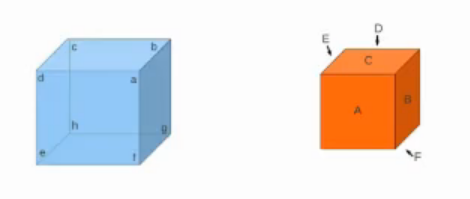
\includegraphics[]{./images/cube.png}
\\
\begin{itemize}
\item $R_0$ : Rotation by $0^{\circ}$, i.e. identity. The cycle index of this permutation has $6$ cycles of length $1$, thus the number of colorings contributed will be $\boxed{x_1^6}$.

\item $R_1$ : Rotation by $180^{\circ}$ w.r.t axis through the center of the opposite faces. (Observe that there are $3$ pairs of such faces). Consider the faces $A, D$. We have observed before that $A, D$ remain in place, and $B, E$ and $C, F$ exchange their places, thus there are $2$ length $1$ cycles and $2$ length $2$ cycles, hence the contributing term will be $x_1^2x_2^2$. As there are $3$ such pairs of faces, the total number of fixed colorings will be $\boxed{3x_1^2x_2^2}$.

\item $R_2$ : Rotation by $90^{\circ}$ w.r.t axis through the center of the opposite faces. Observe that there are $3$ pairs of such faces. Consider the faces $A, D$. They retain their positions, i.e $A \rightarrow A$, $D \rightarrow D$. Now, for the other faces, we have, $C \rightarrow B$, $B \rightarrow F$, $F \rightarrow E$, and $E \rightarrow C$. Thus, there are $2$ length $1$ cycles and $1$ length $4$ cycle, hence the contributing term will be $x_1^2x_4$.As there are $3$ such pairs of faces, the total number of fixed colorings will be $\boxed{3x_1^2x_4}$.

\item $R_3$ : Rotation by $270^{\circ}$ w.r.t axis through the center of the opposite faces. Observe that there are $3$ pairs of such faces. Since this is the exact opposite of the previous case, by symmetry, the total number of fixed colorings will be $\boxed{3x_1^2x_4}$.

\item $R_4$ : Rotation by $180^{\circ}$ w.r.t axis through the midpoints of opposite edges. Observe that there are $6$ pairs of such edges, i.e. $(de, bg),\ (af, ch),\ (ad, hg),\ (cb, ef),\ (ab, eh),\ (cd, fg)$. Suppose we do the rotation w.r.t the edges $(de, bg)$. Then observe that, now $F$ is now the top face, and $A$ occupies the place where $E$ was initially, similarly, $B$ and $D$ swap places. In other words, $C \iff F$, $A \iff E$ and $B \iff D$, i.e. there are $3$ length $2$ cycles. Thus, the contributing term is $x_2^3$. As there are $6$ pairs of edges, the total contributing term will be $\boxed{6 x_2^3}$.

\item $D$ : Diagonal flip by $120^{\circ}$ w.r.t axis through the centers of opposite corners. First, note that there are $4$ pairs of opposite corners. 
Consider the vertex $b$. If we flip the cube along $b$ by $120^{\circ}$, then the face $B \rightarrow C$, i.e. $B$ now occupies the initial position of $C$, $C \rightarrow D$ and $D \rightarrow B$. Thus there is the cycle $B \rightarrow C \rightarrow D \rightarrow B$. Similarly for the other three faces. Thus there are $2$ cycles of length $3$ and hence the contributing term will be $x_3^2$. As there $4$ such pairs of corners, the total term contributed will be $\boxed{4x_3^2}$.

\item $D'$ : Diagonal flip by $240^{\circ}$ w.r.t axis through the centers of opposite corners. First, note that there are $4$ pairs of opposite corners. By symmetry, this is the opposite/complementary operation of the previous one, i.e. flip by $240^{\circ}$ = flip by $120^{\circ}$ in the other direction. Thus, the total term contributed will be $\boxed{4x_3^2}$.
\end{itemize}

Putting all the above together, we get $$P_{G}(x_1, x_2, \ldots x_4) = \frac{1}{24}(x_1^6 + 3x_1^2x_2^2 + 6x_1^2x_4 + 6x_2^3 + 8x_3^2)$$
if we substitute $x_i = 2$ for all $i$, we get 
$$P_{G}(x_1, x_2, \ldots x_4) = \frac{1}{24}(2^6 + 3*2^4 + 6*2^3 + 6*2^3 + 8*2^2) = 10$$
\\

\section{Towards a general formula}
Let us go back to the the example of the square coloring, where $G = \{e, R_{90}, R_{180}, R_{270}, H, V, D, D'\}$, and $G$ as a cycle index permutation is $G = \{(1)(2)(3)(4), (1,2,3,4), (1, 3)(2, 4), (1,4,3,2), (1, 4)(2, 3), (1,2)(3,4), (2,4)(1,3), (1)(3)(2, 4), (2)(4)(1,3)\}$ respectively.
\\
Observe the 2nd, 3rd, and 4th elements of $G$. We know that $R_{90} \circ R_{90} = R_{180}$ i.e. $(1,2,3,4) \circ (1,2,3,4) = (1,3)(2,4)$. Therefore these elements are of the form $g, g^2, g^3$.
\\
Thus, if we have a group whose elements are of the form $G = \{e, g, g^2, \ldots g^k\}$ (called cyclic groups). 
Then the contribution of each term of $g \in G$ will be:
\begin{itemize}
    \item $e - x_1^n$
    \item $g - x_n$
    \item $g^2 - x_{n/2}^2$ and so on
\end{itemize}
Thus, in general, $$P_G(x_1, x_2, \ldots x_m) = \frac{1}{n} \sum_{d|n} \phi(d) x_{d}^{n/d}$$ where $\phi(m)$ is euler's totient function.
\\
\begin{proof}
Consider the element $g^{i}$. Suppose it has a cycle of length $d$. Observe that under this operation, $1 \rightarrow 1+i$, $1+i \rightarrow 1+2i$, \ldots, $1+d*i \rightarrow 1$. This must mean $d*i$ is a multiple of $n$.  Specifically, we must have $d*i = lcm(n, i)$. Using $lcm(n,i) = \frac{n*i}{gcd(n, i)}$, we get $d*i = \frac{n*i}{gcd(n, i)} \implies gcd(n,i) = \frac{n}{d} \implies \boxed{gcd(d, \frac{i*d}{n}) = 1}$.
\\
However there is a bijection between elements of $\phi(d)$ and $i$, because $i = x \frac{n}{d}$ for $x \in \phi(d)$. This implies the number of such $i = \phi(d)$. Thus, the above result shows that all $i$ such that $gcd(d, i) = 1$ contribute $n/d$ cycles of length $d$. Therefore the contribution to the term is $\phi(d) x_{d}^{\frac{n}{d}}$. Hence the proof. 
\end{proof}

Thus, if we have the above formula, the group for the square coloring problem can be represented as $\{e, \sigma, \sigma^2, \ldots, \sigma^{k}, \pi*\sigma, \pi*\sigma^2, \ldots \pi*\sigma^{k-1}\}$. These are called dihedral groups. We discuss more about this in the next lecture.

\input{week10.tex}
\Lecture{Jayalal Sarma}{ 16 November, 2020}{32}{Incidence Algebra and Mobius Inversion Over Posets}{Kaushik Arcot}{$\alpha$}{JS}

\section{Recall}

\begin{theorem}[Stronger PIE]
  \label{stronger PIE}
  Let $f,g:2^{[n]}\longrightarrow \mathbb{R}$ are functions assigning real numbers to subsets of $[n]$ with the property that for any $A\subseteq [n]$

  \[ g(A)=\sum_{S\subseteq A} f(S)\]

  Then,
  \[ f(A) = \sum_{S \subseteq A} (-1)^{|A|-|S|}g(S)\]

\end{theorem}

\textbf{Mobius Inversion of Functions}

$f,g:\mathbb{N} \to \mathbb{R} ~satisfying,$ $\forall n ~g(n) = \sum_{d|n} f(d)  ~~then,$  
$$\forall n ~f(n) = \sum_{d|n} \mu(d)g(\frac{n}{d})$$

	\[
	\mu(d) = \begin{cases} 
	+1 , & ~if~ ~d~ ~is~ ~a~ ~\href{https://en.wikipedia.org/wiki/Square-free_integer}{square-free} ~positive~ ~integer~ ~with~ ~an~ ~even~ ~number~ ~of~ ~prime~ ~factors~~\\
 	-1 , & ~if~ ~d~ ~is~ ~a~ ~square-free~ ~positive~ ~integer~ ~with~ ~an~ ~odd~ ~number~ ~of~ ~prime~ ~factors~~\\
	0 , & otherwise
	\end{cases}
	\]

We can see in both cases that, there is an underlying poset for both the functions. For the first pair of functions, the poset is the Subset Poset, and for the second, it is the divisibilty poset. Our endeavour in this lecture is to further abstract this concept to any poset and acquire tools for algebra within poset functions, and then for Mobius Inversion of functions over posets.

\section{Incidence Algebra of Posets}

Let $P = (X,\le)$ be a poset. Let 

$$ A(P) = \{ f: X \times X \to \mathbb{R} | f(x,y) = 0, \forall x,y \in X  s.t x || y \}$$

Here $x || y$, indicates that x is incomparable to y in the Poset P. \\

Example functions : \\

\textbf{Zero Function} 

$$ O(x,y) = 0 \forall x,y \in X $$

\textbf{Kronecker Delta Function}

$$ \delta(x,y) =  \begin{cases} 
	1 , &  ~if~ ~x~ ~=~ ~y~ \\
	0 , & otherwise
	\end{cases} $$

\textbf{Characteristic Function of Poset}

$$ \zeta(x,y) =  \begin{cases} 
	1 , &  ~if~ ~x~ ~\le~ ~y~ \\
	0 , & otherwise
	\end{cases} $$

\medskip

\textbf{Addition Operator}

Given $f \in A(P)$ , $g \in A(P)$, the '+' operator

$$ (f+g) (x,y) = f(x,y) + g(x,y) $$

If $x || y$, then $f(x,y) = 0$, $g(x,y) = 0$, and hence $(f+g)(x,y) = 0$.
Thus $(f+g) \in A(P)$

\textbf{Remark} : A(P) forms a group with '+' operator as addition.

\medskip
\textbf{Scalar Multiplication}

Given $f \in A(P)$ , $c \in \mathbb{R}$,
$$ (cf)(x,y) = c*f(x,y)$$

If $x||y$, then $f(x,y) = 0$, and so $(cf)(x,y) = 0 $, Hence $(cf) \in A(P)$

\textbf{Remark} : $A(P)$ is closed under addition and scalar multiplication. Thus, $A(P)$ forms a vector space.

\medskip

\textbf{Convolution Operator}

We define the operator '*' over $A(P)$. Given two functions, 
$f,g \in A(P)$, the convolution operator is defined as,

$$ (f*g)(x,y) = \begin{cases} 
	\sum_{z:x\le z \le y} f(x,z)g(z,y), &  ~if~ ~x~ ~\le~ ~y~ \\
	0 , & otherwise
	\end{cases} $$
	
We find if  the following properties of the convolution operator hold or not.

\textbf{Commutative} \\

Convolution operator is not commutative. Assume $x,y \in X$ , such that $x \le y$ and there exists no such z such that $x \le z \le y$. Then,

$$ (f*g)(x,y) = f(x,x)g(x,y) + f(x,y)g(y,y)$$

$$ (g*f)(x,y) = g(x,x)f(x,y) + g(x,y)f(y,y)$$

These two expressions are not always equal. Assume $f(x,x) = 1$, $g(x,y) = 1$, and $f(x,y) = f(y,y) = 0$, $g(x,x) = g(y,y) = 0$. Then, we have

 $(f*g)(x,y) = 1$ and $(g*f)(x,y) = 0$. Therefore, convolution is not commutative.
 
\textbf{Associative}\\

The convolution operator is associative. To prove, assume $f,g,h \in A(P)$. Then,

$$((f*g)*h)(x, y) = \sum_{z: x \le z \le y}(f*g)(x, z) h(z, y)$$

$$ = \sum_{z: x \le z \le y}(\sum_{w: x \le w \le z}f(x, w)g(w, z))h(z, y)$$

By changing the order of the summations, we get,

$$ \sum_{w: x \le w \le z}f(x, w)(\sum_{z : w \le z \le y}g(w, z)h(z, y))$$

$$ = \sum_{w: x \le w \le z}f(x, w) (g*h)(w,y) $$

$$ = (f*(g*h)) (x,y)$$

Hence, convolution is associative.


\textbf{Identity}

\textbf{Claim} : The Kronecker Delta function is the identity function of A(P)

\begin{proof}
For $f \in A(P)$, if $x \le y$,
$$ (f*\delta)(x,y) = \sum_{z:x\le z \le y} f(x,z)\delta(z,y)$$
$$ =  \sum_{z:x\le z < y} f(x,z)\delta(z,y) + f(x,y)\delta(y,y)$$

Given that $z \ne y$, we have $\delta(z,y) = 0$. Thus, $(f*\delta)(x,y)$

$$ = f(x,y)\delta(y,y)$$

$\delta(y,y) = 1$, So

$$ = f(x,y) $$ 

Thus, Kronecker Delta function($\delta$) is the identity function of A(P).

\end{proof}

\section{Inverse of a Function}

The inverse of a function $f \in A(P)$, is a function $g$, such that

$$ (f*g)(x,y) = \delta(x,y)$$

Does the inverse of any $f \in A(P)$ exist ? No. In fact, we check for O(x,y). Let us assume there exists an inverse, Q(x,y) for the zero function. Then,
$$ (O*Q)(x,x) = \sum_{z:x\le z \le x} O(x,z)Q(z,x)$$

$$ = O(x,x)Q(x,x) = 0$$

But $\delta(x,x)$ = 1. Thus, O(x) (zero function) does not have an inverse. Can inverse exist for any other functions ? Yes, we see from this argument that for inverse to exist for $f \in A(P)$, there exists no $x \in X$, such that $f(x,x) = 0$. Infact, we prove next that for $f \in A(P)$, such that $\forall x \in X, f(x,x) \ne 0$, then there exists a unique inverse of f.

\section{Mobius Inversion over Posets}


\begin{lemma}
For any $f \in \mathbb{A}(P)$ such that $\forall x \in X, f(x,x) \ne 0$, there exists $g \in \mathbb{A}(P)$ (which we will call $f^{-1}$) such that $\forall x,y \in X, g \star f = \delta$ where $\delta$ is the Kronecker delta function.
\end{lemma}
\begin{proof}
We will directly write down the function $g$ based on $f$. For incomparable pairs $(x,y)$ we can define $g(x,y) = 0$. This ensures that $g \in \mathbb{A}(P)$. 

For comparable pairs, the function $g$ on input $(x,y)$ is defined based on an induction on a parameter of $\ell(x,y) \in X$. The distance between $x$ and $y$, denoted by $\ell(x,y)$ is said to be $k$, if $\exists z_1, z_2, \ldots z_{k-1}$ such that $x < z_1 < z_2 < \ldots < z_{k-1} < y$ and $\not\exists w_1, w_2, \ldots w_k$ such that $x < w_1 < w_2 < \ldots < w_{k-1} < w_k < y$. In other words, this is the length of the longest directed path from $x$ to $y$ (or vice versa).

Now we are ready to describe the definition of $g$ on comparable pairs $(x,y)$. 

As the base case, when $\ell(x,y) = 0$, we know that, $x=y$, hence we define:

$$g(x,x) = \frac{1}{f(x,x)}$$
Let us quickly check that this indeed satisfies the property that we wanted for inputs of the kind $(x,x)$. That is,
$$(g \star f) (x,x) = \sum_{x \le z \le y} g(x,z)f(z,y) = g(x,x)f(x,x) = 1 = \delta(x,x)$$

To do the definition inductively: let us assume that $g(x,y)$ is defined when $\ell(x,y) \le k$, and we consider a pair $(x,y)$ with distance $k+1$. We define :
$$g(x,y) = \frac{-1}{f(y,y)}\sum_{x \le z < y} g(x,z)f(z,y)$$
Note that this is well-defined since $g(x,z)$ is used in the RHS only for pairs $(x,z)$ with $\ell(x,z) \le k$ and that $f(y,y) \ne 0$ for every $y \in X$.
With this definition :
\begin{eqnarray*}
(g \star f) (x,y) & = & \sum_{x \le z \le y} g(x,z)f(z,y)\\
& = & \sum_{x \le z < y} g(x,z)f(z,y) + g(x,y)f(y,y)\\
& = & \sum_{x \le z < y} g(x,z)f(z,y) + \left(\frac{-1}{f(y,y)}\sum_{x \le z < y} g(x,z)f(z,y)\right) f(y,y) \\
& = & 0 = \delta(x,y)
\end{eqnarray*}
Since $g \in \mathbb{A}(P)$ we have completed the proof.
\end{proof}


\Lecture{Jayalal Sarma}{ 18 November, 2020}{33}{Mobius Inversion Theorem for Posets and Corollaries}{Abhishek Aladahalli}{$\alpha$}{JS}

\noindent In particular the \textbf{zeta function} ($\zeta$)
$$ \zeta (x, y) =  
\begin{cases}
&1 ~~~~\textrm{if} ~~x \le y \\
&0 ~~~~\textrm{otherwise} \\
\end{cases}
$$
has an inverse called the \textbf{Mobius Function} ($\mu$) of the poset.\\

\noindent From the lemma proved above we define Mobius Function as,

\noindent \underline{For $x = y$},
$$g(x,x) = \mu(x,x) = \frac{1}{\zeta (x,x)} = 1$$
$$=> \boxed{\mu(x,x) = 1 ~~ (\textrm{Since} ~\zeta (x,x) = 1)}$$

\noindent \underline{For $x ~ || ~ y$}, (i.e. when $x$ and $y$ are incomparable)
$$g(x,y) = \mu(x,y) = \frac{-1}{\zeta(y,y)}\sum_{x \le z < y} \mu(x,z) \zeta(z,y)$$
$$=> \mu(x,y) = -1\sum_{x \le z < y} \mu(x,z) \zeta(z,y) $$
$$=> \mu(x,y) = -1\sum_{x \le z < y} \mu(x,z) (0) $$
(Since, zeta function ($\zeta$) is $0$ for $x$ and $y$ which are incomparable)
$$=> \boxed{\mu(x,y) = 0}$$

\noindent \underline{For $x \le y$},
$$g(x,y) = \mu(x,y) = \frac{-1}{\zeta(y,y)}\sum_{x \le z < y} \mu(x,z) \zeta(z,y)$$
$$=> \mu(x,y) = -1\sum_{x \le z < y} \mu(x,z) \zeta(z,y) $$
$$=> \mu(x,y) = -1\sum_{x \le z < y} \mu(x,z) (1) ~~~~(\textrm{Since}~~ \zeta(z,y) = 1 ~ \textrm{for} ~z < y)$$
$$=> \boxed{\mu(x,y) = -\sum_{x \le z < y} \mu(x,z)}$$

Hence, Mobius Function is defined as

\begin{center}
    \doublebox{ $\mu (x, y) =  
    \begin{cases}
    &-\sum\limits_{x \le z < y} \mu(x,z) ~~~~~~~~~~~~~~~~~~~~~\textrm{if} ~~x < y \\
    &1 ~~~~~~~~~~~~~~~~~~~~~~~~~~~~~~~~~~~~~~~~~~~~~\textrm{if} ~~ x=y \\
    &0 ~~~~~~~~~~~~~~~~~~~~~~~~~~~~~~~~~~~~~~~~~~~~~\textrm{if x and y are incomparable i.e.} ~~ x ~||~ y\\
    \end{cases}$ }
\end{center}


\noindent Now, Let's consider an example of Divisibility Poset and apply the mobius function on it, 

\begin{center}

\begin{tikzpicture}[auto, node distance=2cm, every loop/.style={}, thick,main node/.style={circle,draw,font=\sffamily\Large\bfseries}]

\node[main node] (1) {90};
\node[main node] (2) [below left of=1] {30};
\node[main node] (3) [right of=2] {45};
\node[main node] (4) [right of=3] {18};
\node[main node] (5) [below left of=2] {10};
\node[main node] (6) [right of=5] {15};
\node[main node] (7) [right of=6] {6};
\node[main node] (8) [right of=7] {9};
\node[main node] (9) [below right of=5] {5};
\node[main node] (10) [right of=9] {2};
\node[main node] (11) [right of=10] {3};
\node[main node] (12) [below left of=11] {1};


\path[every node/.style={font=\sffamily\small}]
    (1) edge node [] {} (4)
        edge node [] {} (3)
        edge node [] {} (2)
    (2) edge node [] {} (5)
        edge node [] {} (6)
        edge node [] {} (7)
    (3) edge node [] {} (6)
        edge node [] {} (8)
    (4) edge node [] {} (7)
        edge node [] {} (8)
    (5) edge node [] {} (9)
        edge node [] {} (10)
    (6) edge node [] {} (9)
        edge node [] {} (11)
    (7) edge node [] {} (10)
        edge node [] {} (11)
    (8) edge node [] {} (11)
    (9) edge node [] {} (12)
    (10) edge node [] {} (12)
    (11) edge node [] {} (12);

\end{tikzpicture}
    
\end{center}

\begin{align*}
\textrm{For} ~~(x,y) = (1,1),\\
    \mu (x,y) &= \mu (1,1)\\
=>  \mu (1,1) &= 1~~~~~~~~~~~(\because x = y)\\\\
\textrm{For} ~~(x,y) = (1,2),\\
    \mu (x,y) &= \mu (1,2)\\
=>  \mu (1,2) &= -\sum\limits_{1 \le z < 2} \mu(1,z)    ~~~~~~~\textrm{(By definition of mobius function)}\\
    &= - \mu(1,1)\\
=>  \mu(1,2) &= -1\\\\
\textrm{Similarly for} ~~(x,y) = (1,3),\\
=> \mu(1,3) &= -1\\\\
\textrm{Similarly for} ~~(x,y) = (1,5),\\
=> \mu(1,5) &= -1\\
\end{align*}

Thus, In general for a prime number $p$,

\begin{center}
    \doublebox{
    $\mu(1,p) = -1$
    }
\end{center}

Now,
\begin{align*}
\textrm{For} ~~(x,y) = (1,10),\\
    \mu (x,y) &= \mu (1,10)\\
=>  \mu (1,10) &= -\sum\limits_{1 \le z < 10} \mu(1,z)    ~~~~~~~\textrm{(By definition of mobius function)}\\
    &= - (\mu(1,1) + \mu(1,2) + \mu(1,5)) \\
=>  \mu(1,10) &= 1\\\\
\textrm{Similarly for} ~~(x,y) = (1,15),\\
=> \mu(1,15) &= 1\\\\
\textrm{Similarly for} ~~(x,y) = (1,6),\\
=> \mu(1,6) &= 1\\
\end{align*}

Thus, In general for prime numbers $p$ and $q$ ,
\begin{center}
    $\mu(1,p q) = -(\mu(1,1) + \mu(1,p) + \mu(1,q))$\\
    $=>$\doublebox{
    $\mu(1,p q) = 1$
    }
\end{center}

\noindent Now,
\begin{align*}
\textrm{For} ~~(x,y) = (1,9),\\
    \mu (x,y) &= \mu (1,9)\\
=>  \mu (1,9) &= -\sum\limits_{1 \le z < 9} \mu(1,z)    ~~~~~~~\textrm{(By definition of mobius function)}\\
    &= - (\mu(1,1) + \mu(1,3)) \\
=>  \mu(1,9) &= 0\\
\end{align*}

Thus, In general for a prime number $p$,

\begin{center}
    \doublebox{
    $\mu(1,p^2) = 0$
    }
\end{center}

\noindent Now,
\begin{align*}
\textrm{For} ~~(x,y) = (1,45),\\
    \mu (x,y) &= \mu (1,45)\\
=>  \mu (1,45) &= -\sum\limits_{1 \le z < 45} \mu(1,z)    ~~~~~~~\textrm{(By definition of mobius function)}\\
    &= - (\mu(1,1) + \mu(1,3) + \mu(1,5) + \mu(1,9) + \mu(1,15)) \\
=>  \mu(1,45) &= 0\\\\
\textrm{Similarly for} ~~(x,y) = (1,18),\\
=> \mu(1,18) &= 0\\
\end{align*}

Thus, In general for prime numbers $p$ and $q$,

\begin{center}
    $\mu(1,p^2 q) = -(\mu(1,1) + \mu(1,p) + \mu(1,q) + \mu(1,p q) + \mu(1,p^2) )$
    \\
    $=>$\doublebox{
    $\mu(1,p^2 q) = 0$
    }
\end{center}

\noindent Now,
\begin{align*}
\textrm{For} ~~(x,y) = (1,30),\\
    \mu (x,y) &= \mu (1,30)\\
=>  \mu (1,30) &= -\sum\limits_{1 \le z < 30} \mu(1,z)    ~~~~~~~\textrm{(By definition of mobius function)}\\
    &= - (\mu(1,1) + \mu(1,3) + \mu(1,5) + \mu(1,2) + \mu(1,6) + \mu(1,10) + \mu(1,15)) \\
=>  \mu(1,30) &= -1\\
\end{align*}

Thus, In general for prime numbers $p$, $q$ and $r$,

\begin{center}
    $\mu(1,p q r) = -(\mu(1,1) + \mu(1,p) + \mu(1,q) + \mu(1,p q) + \mu(1,q r) + \mu (1, p r) )$
    \\
    \doublebox{
    $\mu(1,p q r) = 1$
    }
\end{center}

Therefore In general, The mobius function for the divisibility poset turns out to be,

\begin{center}
    \doublebox{ $\mu (d)
    \begin{cases}
        &= +1 ~~~~~~~~~~~~\textrm{If $d$ is a product of even number of primes}\\
        &= -1 ~~~~~~~~~~~~\textrm{If $d$ is a product of odd number of primes}\\
        &= 0 ~~~~~~~~~~~~~\textrm{Otherwise}\\
    \end{cases}
    $
    }
\end{center}

\section{Mobius Inversion theorem over Posets}

\textbf{Assumption :}

\noindent In the poset $X$, there is a unique $m$ such that $\forall x \in X$, $m \le x$

\begin{theorem}

For a poset $X$, if $f$ is a function $f: X \rightarrow \mathbb{R}$ and $g$ is a function $g: X \rightarrow \mathbb{R}$ such that,
$$\forall a \in X, ~~~~~~~~g(a) = \sum_{x \le a} f(x)$$ 
then
$$\boxed{\forall a \in X, ~~~~~~~~f(a) = \sum_{x \le a} \mu(x,a) g(x)}$$
where $\mu$ is the mobius function of the poset.
\end{theorem}

\begin{proof}

As from the assumption, let $m$ be the unique minimal element of the poset $X$.

\noindent And let $f$ and $g$ be the functions defined as above such that 

$$\forall a \in X, ~~g(a) = \sum\limits_{x \le a} f(x)  ~~~~~~~~~(1)$$

\noindent Now, we define two functions $F(x,y)$ and $G(x,y)$ such that,

\begin{Parallel}[v]{0.48\textwidth}{0.48\textwidth}
\ParallelLText{
\begin{align*}
   & \forall a \in X ,\\
   & F(m,a) = f(a)\\
   & G(m,a) = g(a)\\
\end{align*}}
\ParallelRText{
\begin{align*}
   & \textrm{For all other}~ x ~\textrm{and} ~ y ~ \textrm{where} ~ x \ne m,\\
   & F(x,y) = 0\\
   & G(x,y) = 0\\
\end{align*}
}
  \ParallelPar
\end{Parallel}

\noindent Thus, By Incidence Algebra $F,G \in A(P)$ for $P(X,\le)$.\\

\noindent \textbf{Claim :}
$$\boxed{G = F \star \zeta ~~\textrm{where $\zeta$ is the zeta function.}}$$

\noindent \underline{Note:} Through this claim we can show that $F = G \star \mu$ (where $\mu$ is the mobius function) and thus proving the theorem.\\


\noindent \textbf{Proof for the claim :}

\noindent Consider $G(x,y)$,

\textbf{Case 1 : $\forall a \in X$}
\begin{align*}
    G(m,a) &= g(a)\\
    &= \sum_{x \le a} f(x) ~~~~~~~~~~~~~~~~ \textrm{( $\because~$ from (1))}\\
    &= \sum_{m \le x \le a} F(m,x) ~~~~~~~~ \textrm{($\because~$from definition of $F(x,y)$)}\\
    &= \sum_{m \le x \le a} F(m,x) \zeta(x,a) ~~~~~~\textrm{($\because \zeta (x,a) = 1, \forall x \le a$ )}
\end{align*}
$$=> \boxed{G(m,a) = F \star \zeta (m,a)} ~~~~~~~~~~~~ \textrm{( $\because~$ By defintion of convolution ($\star$))}$$

\textbf{Case 2 :} For all other $x$ and $y$ where $x \ne m$
\begin{align*}
    G(x,y) &= 0\\
    &= \sum_{x \le z \le y} F(x,z) \zeta(z,y) ~~~~~~\textrm{($\because F(x,z) = 0, \forall x \ne m$ )}
\end{align*}
$$=> \boxed{G(x,y) = F \star \zeta (x,y)} ~~~~~~~~~~~~ \textrm{($\because~$By defintion of convolution ($\star$))}$$

\noindent Hence, The claim $G = F \star \zeta $ is true.\\

\noindent Thus, By definition
$$\boxed{F = G \star \mu}$$

\noindent Therefore, $\forall a \in X$,
\begin{align*}
    F(m,a) &= \sum_{m \le x \le a} G(m,x) \mu(x,a) ~~~~~~~~ \textrm{($\because~$By defintion of convolution ($\star$))}\\
 => f(a)  &=\sum_{x \le a} g(x) \mu(x,a) ~~~~~~~~ \textrm{($\because~$From defintion of $F(m,a) = f(a), G(m,x) = g(x)$)}
\end{align*}

\noindent Thus,
\begin{center}
    \doublebox{$\forall a \in X, ~~~~~~~~f(a)  = \sum\limits_{x \le a} \mu(x,a) g(x)$}
\end{center}

Hence Proved.\\

\end{proof}

\subsection{Corollary}

\noindent \underline{\textbf{Application of Mobius Inversion theorem on Subset Poset}}\\

\noindent For the subset poset we will show, if $f$ and $g$ are functions defined from subsets to real numbers (i.e. 
$f: 2^{[n]} \rightarrow \R$ , $g: 2^{[n]} \rightarrow \R $ ) such that
$$\forall A \subseteq [n], ~~~~~ g(A) = \sum_{S \subseteq A} f(S) $$
then
$$\boxed{\forall A \subseteq [n], ~~~~~ f(A) = \sum_{S \subseteq A} (-1)^{|A|- |S|}g(S) } $$

\noindent \textbf{Claim :} For $X \subseteq [n]$ and $Y \subseteq [n]$,
$$ \mu (X,Y) = 
\begin{cases}
    &0 ~~~~~~~~~~~~~~~~~~~~~~~~~~~~\textrm{if $~X \nsubseteq Y$}\\
    &(-1)^{|Y| - |X|} ~~~~~~~~~~\textrm{if $~X \subseteq Y$}\\
\end{cases}
$$
\underline{\textsf{Note :}} If we prove the claim to be true then the above subset poset can directly be shown as a corollary of the mobius inversion theorem by substituting the value of $\mu$.\\

\noindent \textbf{Proof for the claim :} 

\noindent We will apply Induction on $|Y|-|X|$ for $X \subseteq Y$.\\

\noindent \underline{Base step}, For $|Y| - |X| = 0$ i.e. $X = Y$
\begin{align*}
    \mu (X,Y) &= \mu(X,X)\\
    => \mu (X,Y) &= 1  ~~~~~~~~~~\textrm{($\because X \subseteq X ~$ and $~\mu (X,X) = 1$ )}\\
    => \mu (X,Y) &= (-1)^{0} = (-1)^{|Y| - |X|}
\end{align*}

\noindent \underline{Induction step}, Assume it's true for $|Y| - |X| \le k$. Now, we need to prove it's also true for $|Y| - |X| = k + 1$.\\

\noindent Thus, Consider $\mu (X,Y)$ for $|Y| - |X| = k + 1$,
\begin{align*}
    \mu (X,Y) &= - \sum_{X \subseteq Z \subset Y} \mu (X,Z) ~~~~~~~~~~~~~\textrm{($\because X < Y~$ and by definition of mobius function )}\\
 => \mu (X,Y) &= - \sum_{X \subseteq Z \subset Y} (-1)^{|Z|-|X|} ~~~~~~~\textrm{($\because |Z| - |X| \le k~$ and it's assumed true for $|Y| - |X| \le k$)}\\
 => \mu (X,Y) &= - \sum_{X \subseteq Z \subseteq Y} (-1)^{|Z|-|X|} + (-1)^{|Y| - |X|} ~~~~~~~\textrm{($\because~$Adding and subtracting the subset $Y$)}
\end{align*}
$$=> \boxed{\mu (X,Y) = - \sum_{X \subseteq Z \subseteq Y} (-1)^{|Z|-|X|} + (-1)^{|Y| - |X|}} ~~~~~~\textrm{(1)}$$

\noindent Now, we will show that 1st term in the R.H.S goes to 0 by using a combinatorial argument.\\

\noindent So, For given $X, Y \subseteq [n]$ and $X \subseteq Y$,
\begin{align*}
    \sum_{X \subseteq Z \subseteq Y} (-1)^{|Z|-|X|} &= \sum_{k} \sum_{\substack{X \subseteq Z \subseteq Y\\ |Z| - |X| = k}} (-1)^k ~~~~~\textrm{(By rewriting the summation based on the size of $|Z| - |X|$)}\\
    &= \sum_{k} (-1)^k {n \choose k} ~~~~~~~~~\textrm{($\because~$ Number of ways of choosing such a subset $|Z|$ is ${n \choose k}$) }\\
    &= 0 ~~~~~~~~~~~~~~~~~~~~~~~~~~\textrm{($\because ~$ Signed summation of binomial coefficients is $0$)}\\
=> \sum_{X \subseteq Z \subseteq Y} (-1)^{|Z|-|X|} &= 0\\
\end{align*}
Therefore, Equation (1) becomes,\\

\begin{center}
    \doublebox{
$\mu (X,Y) = (-1)^{|Y|-|X|}$
}
\end{center}

Hence Proved.\\

\noindent Thus, from this definition of $\mu$ and the theorem of Mobius Inversion, the corollary on the subset poset follows that ,\\

\noindent \textbf{Corollary :} If $f$ and $g$ are functions defined from subsets to real numbers (i.e. 
$f: 2^{[n]} \rightarrow \R$ , $g: 2^{[n]} \rightarrow \R $ ) such that
$$\forall A \subseteq [n], ~~~~~ g(A) = \sum_{S \subseteq A} f(S) $$
then
\begin{center}
    \doublebox{
    $\forall A \subseteq [n], ~~~~~ f(A) = \sum\limits_{S \subseteq A} (-1)^{|A|- |S|}g(S) $
    }
\end{center}











\Lecture{Jayalal Sarma}{ 19 November, 2020}{34}{More Applications of Structure of Partial Orders, Fixed Point Theorems}{Kaushik Arcot, Abhishek Aladahalli}{$\alpha$}{JS}

\section{Equinumerous Sets and Bijections}

We define Cardinality using the concept of Bijections and Equinumerous sets.
\begin{theorem}
Two sets A, B are equinumerous or equal in cardinality iff there
exists a bijection $f: A \to B$. Or,\\

$ |A| = |B| \Leftrightarrow \exists$ bijection $f:A \to B $ \\

\end{theorem}

\textbf{Example of Equinumerous sets and Bijections}\\

\textbf{Even Numbers and $\mathbb{N}$}\\

$f:\mathbb{E} \to \mathbb{N}$,  $f(x) = x/2$

Is a bijection from even numbers to Natural Numbers.\\

The Noton of Cardinality arises from the fact that these Equinumerous sets divide the Subset Partial Order into different equivalence classes and each of those classes correspond to different cardinalities. \\

So to prove that two sets are equinumerous sets, we need to prove there exists a bijection between the two sets. To prove that there exists a bijection between two sets, we can just prove that there exists an injection in both directons.

\begin{theorem}[Cantor Schroeder Bernstein Theorem]
$A,B \subseteq U$ ,$\exists f:A \to B, g:B \to A$ are injections $\implies \exists h:A \to B$ which is a bijection 
\end{theorem}

This theorem is intuitive in finite sets, but to prove for infinite sets, we need some more tools that concern posets and cardinality.

\section{Knaster-Tarski Fixed point theorem}

To prove this theorem, we need to understand some properties.

\textbf{Fixed Point of a Function}\\
Let $f: X \to X$, be a function. Then, a point $x \in X$, is said to be a fixed point of function $f$ if $f(x) = x$.

\textbf{Preserving Order of Posets}

Let $P(X,\le)$ be a poset. Then any function $f: X \to X$ is said to preserve order if 
$$ \forall x,y \in X, x \le y \implies f(x)  \le f(y) $$

\textbf{Upper Bound of a Set}

Let $P(X,\le)$ be a poset, and $A \subseteq X$, then the upper bound of set A is defined as 

$$ UB(A) = \{x \in X | \forall y \in A, y \le x\} $$

\textbf{Least Upper Bound of a Set}

Let $P(X,\le)$ be a poset, and $A \subseteq X$, then the least upper bound of set A is defined from the upper bound set, as the least element in the upper bound set of A.

$$ LUB(A) = \{x  | \forall y \in UB(A), x \le y\} $$

\textbf{Complete Partial Order}

A partial order $P(X,\le)$ is set to be a complete partial order, if $\forall A \subseteq X$ , $\exists LUB(A)$

\medskip


We can understand the notion of a complete partial order using the subsets partial order. Let $P(X,\le)$, be the subsets partial order, where $X = 2^{[n]}$. Then, let $A \subseteq X$, be a subset of X, which is a set of subsets of $[n]$. Assume, $A = \{A_1,A_2,...A_k\}$, and S =  $\bigcup_{i=1}^{k} A_{i}$ forms the LUB of the set A. We know that $\forall i \in [k], A_i \le S$, (because $A_i$ is a subset of S, S is the union of all $A_i$'s). And it is the lowest upper bound, as any element missing from $S$, will be present in one of the $A_i$'s.

Now, we're ready to prove the Knaster-Tarski Theorem.

\begin{theorem}[Knaster-Tarski Fixed point theorem]
Let $P(X,\le)$ be a complete partial order, and let $f: X \to X$, be a function that preserves the order on the partial order P. Then $f$ has a fixed point.
\end{theorem}

\begin{proof}
Consider the set $A = \{x | x \le f(x)\}$. Assume that A is non-empty. This is possible when X has a least element in P. Then, for that least element $x \in X$, $\forall y \in X, x \le y$. And $f(x) \in X$, thus, $x \le f(x)$, and therefore $x \in A$. \\

\textbf{Observation} If $x \in A$, then $f(x) \in A$. \\
$x \in A$. $\implies x \le f(x)$. As f preserves order,\\
$ \implies f(x) \le f(f(x) $. Let f(x) = z, then \\
$z \le f(z)$. Thus, $z \in A$. $\implies f(x) \in A$.\\

Since the partial order is complete, and $A \subseteq X$, there exists an LUB(A). Let

$$ y = LUB(A)$$

Consider, $\forall x \in A$. As y is LUB,\\
$x \le y$ , As f preserves order\\
$ f(x) \le f(y) $. Becasue $x \in A$, \\

$x \le f(x) \le f(y), \forall x \in A$ \\

This implies that $f(y)$ is an upper bound of A. Since $y$ is the LUB of A,
$$y \le f(y) $$

By the property of A, it is clear that $y \in A$. And because $y \in A$, and from the observation proven above, we have that $f(y) \in A$. \\

Since $f(y) \le A$, and y is LUB(A) of A, we have that
$$ f(y) \le y $$

So, we have,
$$ f(y) \le y \And y \le f(y) $$.

By the anti-symmetry of the relation $\le$ in the partial order, we have 
$$f(y) = y $$

So, we have $y$ as the fixed point.\\

Hence proved.

\end{proof}


\section{Cantor-Schroeder-Bernstein Theorem}

\begin{theorem}[Cantor Schroeder Bernstein Theorem]
$A,B \subseteq U$ ,$\exists f:A \to B, g:B \to A$ that are injections $\implies \exists h:A \to B$ which is a bijection.
\end{theorem}

\begin{proof}

We find a $H \subseteq A$, and we build a function h, such that
$$ h |_H = f \And h|_{\bar H} = g $$

Then, we prove that H is a bijection.

\textbf{Claim} For $H \subseteq A$, if $g( \bar{f(H)} ) = \bar H$ then by  the above definition, h is a bijection. \\

Or, we have to find an H such that $H = \bar{g(\bar{f(H)})}$ \\


First, we find an H such that this claim is satisfied, and then we prove the claim. \\

We define the following function on the subset partial order of A.\\

$\tau : 2^{[A]} \to 2^{[A]}$, such that for any $T \subset A$,

$$ \tau(T) = \bar{g(\bar{f(T)})}$$

We will prove the properties of preserving order and completeness of this Partial Order. \\

We know that the partial order is complete, as it is a subset poset. \\

For preserving order, assume $S \subset T$. . By applying f on both sides, we have $f(S) \subset f(T)$. \\

Taking complement, we have $\bar{f(T)} \subset \bar{f(S)}$.\\

As g is a function from B to A, and $f(x) \in B \forall x \in A$, applying g on both sides, we get \\

$$ g(\bar{f(T)}) \subset g(\bar{f(S)})$$

Again taking complement, we get 

$$ \bar{g(\bar{f(S)})} \subset \bar{g(\bar{f(T)})} $$

So, $\tau(S) \subset \tau(T)$. Hence $\tau$ preserves order.\\

Because $\tau$ preserves order and and $P = ([A],\le)$ is a complete poset, we have that there exists a fixed point for $\tau$. Therefore

$$ \exists H \subset A, \bar{g(\bar{f(H)})} = H $$

Now that we have arrived at an H, we now need to prove that $h$ is a bijection. We need to prove three parts. \\

\textbf{Well-defined} \\
h is well defined. $\forall x \in A$, if $x \in H$, the output of $h$ is f(x). Otherwise, as $g$ is injective, and $\bar H = g(\bar{f(H)})$, and so $\bar H \subseteq g(B)$, and $g^{-1}(x)$ is defined $\forall x \in g(B)$, and subsequently in $\bar H$. So $\forall x \in A$, h(x) is well defined.

\textbf{Injective}\\
We need to prove $\forall x,y \in A$, $x \ne y \implies h(x) \ne h(y)$.

\textsf{Case 1} : $x \in H \And y \in H$\\

$\forall x \in H$, $h(x) = f(x)$. Therefore, $x \ne y \implies f(x) \ne f(y) \implies h(x) \ne h(y) $


\textsf{Case 2}: $x \in \bar H \And y \in \bar H$

$\forall x \in \bar H$, $h(x) = g^{-1}(x)$.  Since g is injective, $g^{-1}$  is well-defined, and thus $g^{-1}(x) \ne g^{-1}(y) \implies h(x) \ne h(y)$

\textsf{Case 3} : $x \in H \And y \in \bar H$
For $x \in H$, $h(x) = f(x)$\\
For $y \in \bar H$, $h(y) = g^{-1}(y)$ \\

We need to prove $h(x) \ne g^{-1}(y)$ \\

We know, $g(\bar{f(H)}) = \bar H $. As $g^{-1}$ is well defined, $\implies g^{-1}(\bar H) \subseteq \bar{f(H)}$ \\. Therefore, $g^{-1}(H) \nsubseteq f(H)$. Moreover, as $g^{-1}(\bar H) \subseteq \bar{f(H)}$, $ \nexists u \in \bar H$, such that $g^{-1}(u) \in f(H)$.
Thus, for $x \in H \And y \in \bar H$, $g^{-1}(y) \ne f(x)$. Hence proved.

\textbf{Surjective} \\
To prove, $range(h) = B$. That is, $\forall y \in B, \exists x \in A$, such that $h(x) = y$. Assume, $y \in f(H)$. Given that $\forall x in H, h(x) = f(x)$, and because $y \in f(H)$, $\exists x, f(x) = y$.

Now, for $x \in \bar{f(H)}$. We know,

\begin{equation} \label{eqn:1} \bar H = g(\bar{f(H)}) \end{equation}

And that $g^{-1}(x)$ is defined $\forall x \in \bar H$ (already proved). Since $g^{-1}$ is obviously injective ( if $x \ne y$ and  $g^{-1}(x) = g^{-1}(y) = a$, then $g(a)$ is not defined), we can apply $g^{-1}$ on both sides of \ref{eqn:1}, to get 

$$ g^{-1}(\ba   r H) \subseteq \bar{f(H)}$$

As $g{-1}$ is injective, and we know that $|\bar H| = g(\bar{f(H)})$, both the sets are of the same size, thus,
$$ g^{-1}(\bar H) = \bar{f(H)}$$.

$\forall x \in \bar{f(H)}$, we have a pre-image in $g^{-1}(\bar H)$. Hence, h is surjective.

From the three parts, we have proven that $h : A \to B$, is a bijective function, constructed from $f : A \to B$ and $g : B \to A$, two injective functions.

\end{proof}

%\input{problemsets.tex}

\newpage
\chapter{Supplementary Material}

\section{Curiosity Collection}

Here we list down all the "out of curious" questions that we discussed (sometimes even not discussed) in the class (and hence in this document).
\includecollection{curious.tmp}

\newpage
\section{Exercises}
\setcounter{excount}{0}
\includecollection{ex.tmp}

\newpage

%% Convention : Call all problem set collection names with psXX.tmp This helps in managing the auxillary files created by collect package.Give back reference to problems in lectures.
%\def\psetbackref{0}

\section{Problem Sets}

\subsection{~Problem Set \#1}
\begin{enumerate}[(1)]
  \includecollection{ps1.tmp}
\end{enumerate}

%\newpage
%\section{~Problem Set \#2}
%
%\begin{enumerate}[(1)]
%\includecollection{ps2.tmp}
%\end{enumerate}
%
%\newpage
%\section{~Problem Set \#3}
%
%\begin{enumerate}[(1)]
%\includecollection{ps3.tmp}
%\end{enumerate}
%
%\newpage
%\section{~Problem Set \#4}
%
%\begin{enumerate}[(1)]
%\includecollection{ps4.tmp}
%\end{enumerate}

\bibliographystyle{apalike}
\bibliography{references}

\end{document}

